
%(BEGIN_QUESTION)
% Copyright 2006, Tony R. Kuphaldt, released under the Creative Commons Attribution License (v 1.0)
% This means you may do almost anything with this work of mine, so long as you give me proper credit

Plot a graph of an RTD's resistance over a temperature range of 0$^{o}$ C to 200$^{o}$ C.  Assume a 100 $\Omega$ RTD with an European alpha value.

$$
\includegraphics[width=15.5cm]{i00412x01.eps}$$

Then, plot a graph of a bridge circuit's voltage output containing the same RTD (100 $\Omega$, American $\alpha$), as its temperature changes from 0$^{o}$ C to 200$^{o}$ C:

$$
\includegraphics[width=15.5cm]{i00412x03.eps}$$

$$
\includegraphics[width=15.5cm]{i00412x04.eps}$$

Compare these two graphs, then comment on the behavior of RTDs both inside and outside of a bridge circuit.

\vskip 20pt \vbox{\hrule \hbox{\strut \vrule{} {\bf Suggestions for Socratic discussion} \vrule} \hrule}

\begin{itemize}
\item{} Explain how a {\it computer spreadsheet program} such as Microsoft Excel might be useful in graphing the results of this circuit.
\end{itemize}

\underbar{file i00412}
%(END_QUESTION)





%(BEGIN_ANSWER)

$$\includegraphics[width=15.5cm]{i00412x02.eps}$$

$$\includegraphics[width=15.5cm]{i00412x05.eps}$$

The contrast is obvious.  I'll let you reach your own conclusions!

%(END_ANSWER)





%(BEGIN_NOTES)

\noindent
Data points for graphs:

\vskip 10pt
\begin{itemize}
\item{} T = 0$^{o}$ C ; R = 100 $\Omega$; $V_{out}$ = 0 mV 
\item{} T = 50$^{o}$ C ; R = 119.6 $\Omega$; $V_{out}$ = 2.2313 mV 
\item{} T = 100$^{o}$ C ; R = 139.2 $\Omega$; $V_{out}$ = 4.0970 mV 
\item{} T = 150$^{o}$ C ; R = 158.8 $\Omega$; $V_{out}$ = 5.6801 mV 
\item{} T = 200$^{o}$ C ; R = 178.4 $\Omega$; $V_{out}$ = 7.0402 mV 
\end{itemize}
%INDEX% Measurement, temperature: RTD

%(END_NOTES)


